\documentclass[]{article}
\usepackage{lmodern}
\usepackage{amssymb,amsmath}
\usepackage{ifxetex,ifluatex}
\usepackage{fixltx2e} % provides \textsubscript
\ifnum 0\ifxetex 1\fi\ifluatex 1\fi=0 % if pdftex
  \usepackage[T1]{fontenc}
  \usepackage[utf8]{inputenc}
\else % if luatex or xelatex
  \ifxetex
    \usepackage{mathspec}
  \else
    \usepackage{fontspec}
  \fi
  \defaultfontfeatures{Ligatures=TeX,Scale=MatchLowercase}
\fi
% use upquote if available, for straight quotes in verbatim environments
\IfFileExists{upquote.sty}{\usepackage{upquote}}{}
% use microtype if available
\IfFileExists{microtype.sty}{%
\usepackage{microtype}
\UseMicrotypeSet[protrusion]{basicmath} % disable protrusion for tt fonts
}{}
\usepackage[margin=1in]{geometry}
\usepackage{hyperref}
\hypersetup{unicode=true,
            pdftitle={PS 1 QTM 200},
            pdfauthor={Robert Song},
            pdfborder={0 0 0},
            breaklinks=true}
\urlstyle{same}  % don't use monospace font for urls
\usepackage{color}
\usepackage{fancyvrb}
\newcommand{\VerbBar}{|}
\newcommand{\VERB}{\Verb[commandchars=\\\{\}]}
\DefineVerbatimEnvironment{Highlighting}{Verbatim}{commandchars=\\\{\}}
% Add ',fontsize=\small' for more characters per line
\usepackage{framed}
\definecolor{shadecolor}{RGB}{248,248,248}
\newenvironment{Shaded}{\begin{snugshade}}{\end{snugshade}}
\newcommand{\AlertTok}[1]{\textcolor[rgb]{0.94,0.16,0.16}{#1}}
\newcommand{\AnnotationTok}[1]{\textcolor[rgb]{0.56,0.35,0.01}{\textbf{\textit{#1}}}}
\newcommand{\AttributeTok}[1]{\textcolor[rgb]{0.77,0.63,0.00}{#1}}
\newcommand{\BaseNTok}[1]{\textcolor[rgb]{0.00,0.00,0.81}{#1}}
\newcommand{\BuiltInTok}[1]{#1}
\newcommand{\CharTok}[1]{\textcolor[rgb]{0.31,0.60,0.02}{#1}}
\newcommand{\CommentTok}[1]{\textcolor[rgb]{0.56,0.35,0.01}{\textit{#1}}}
\newcommand{\CommentVarTok}[1]{\textcolor[rgb]{0.56,0.35,0.01}{\textbf{\textit{#1}}}}
\newcommand{\ConstantTok}[1]{\textcolor[rgb]{0.00,0.00,0.00}{#1}}
\newcommand{\ControlFlowTok}[1]{\textcolor[rgb]{0.13,0.29,0.53}{\textbf{#1}}}
\newcommand{\DataTypeTok}[1]{\textcolor[rgb]{0.13,0.29,0.53}{#1}}
\newcommand{\DecValTok}[1]{\textcolor[rgb]{0.00,0.00,0.81}{#1}}
\newcommand{\DocumentationTok}[1]{\textcolor[rgb]{0.56,0.35,0.01}{\textbf{\textit{#1}}}}
\newcommand{\ErrorTok}[1]{\textcolor[rgb]{0.64,0.00,0.00}{\textbf{#1}}}
\newcommand{\ExtensionTok}[1]{#1}
\newcommand{\FloatTok}[1]{\textcolor[rgb]{0.00,0.00,0.81}{#1}}
\newcommand{\FunctionTok}[1]{\textcolor[rgb]{0.00,0.00,0.00}{#1}}
\newcommand{\ImportTok}[1]{#1}
\newcommand{\InformationTok}[1]{\textcolor[rgb]{0.56,0.35,0.01}{\textbf{\textit{#1}}}}
\newcommand{\KeywordTok}[1]{\textcolor[rgb]{0.13,0.29,0.53}{\textbf{#1}}}
\newcommand{\NormalTok}[1]{#1}
\newcommand{\OperatorTok}[1]{\textcolor[rgb]{0.81,0.36,0.00}{\textbf{#1}}}
\newcommand{\OtherTok}[1]{\textcolor[rgb]{0.56,0.35,0.01}{#1}}
\newcommand{\PreprocessorTok}[1]{\textcolor[rgb]{0.56,0.35,0.01}{\textit{#1}}}
\newcommand{\RegionMarkerTok}[1]{#1}
\newcommand{\SpecialCharTok}[1]{\textcolor[rgb]{0.00,0.00,0.00}{#1}}
\newcommand{\SpecialStringTok}[1]{\textcolor[rgb]{0.31,0.60,0.02}{#1}}
\newcommand{\StringTok}[1]{\textcolor[rgb]{0.31,0.60,0.02}{#1}}
\newcommand{\VariableTok}[1]{\textcolor[rgb]{0.00,0.00,0.00}{#1}}
\newcommand{\VerbatimStringTok}[1]{\textcolor[rgb]{0.31,0.60,0.02}{#1}}
\newcommand{\WarningTok}[1]{\textcolor[rgb]{0.56,0.35,0.01}{\textbf{\textit{#1}}}}
\usepackage{graphicx,grffile}
\makeatletter
\def\maxwidth{\ifdim\Gin@nat@width>\linewidth\linewidth\else\Gin@nat@width\fi}
\def\maxheight{\ifdim\Gin@nat@height>\textheight\textheight\else\Gin@nat@height\fi}
\makeatother
% Scale images if necessary, so that they will not overflow the page
% margins by default, and it is still possible to overwrite the defaults
% using explicit options in \includegraphics[width, height, ...]{}
\setkeys{Gin}{width=\maxwidth,height=\maxheight,keepaspectratio}
\IfFileExists{parskip.sty}{%
\usepackage{parskip}
}{% else
\setlength{\parindent}{0pt}
\setlength{\parskip}{6pt plus 2pt minus 1pt}
}
\setlength{\emergencystretch}{3em}  % prevent overfull lines
\providecommand{\tightlist}{%
  \setlength{\itemsep}{0pt}\setlength{\parskip}{0pt}}
\setcounter{secnumdepth}{0}
% Redefines (sub)paragraphs to behave more like sections
\ifx\paragraph\undefined\else
\let\oldparagraph\paragraph
\renewcommand{\paragraph}[1]{\oldparagraph{#1}\mbox{}}
\fi
\ifx\subparagraph\undefined\else
\let\oldsubparagraph\subparagraph
\renewcommand{\subparagraph}[1]{\oldsubparagraph{#1}\mbox{}}
\fi

%%% Use protect on footnotes to avoid problems with footnotes in titles
\let\rmarkdownfootnote\footnote%
\def\footnote{\protect\rmarkdownfootnote}

%%% Change title format to be more compact
\usepackage{titling}

% Create subtitle command for use in maketitle
\providecommand{\subtitle}[1]{
  \posttitle{
    \begin{center}\large#1\end{center}
    }
}

\setlength{\droptitle}{-2em}

  \title{PS 1 QTM 200}
    \pretitle{\vspace{\droptitle}\centering\huge}
  \posttitle{\par}
    \author{Robert Song}
    \preauthor{\centering\large\emph}
  \postauthor{\par}
      \predate{\centering\large\emph}
  \postdate{\par}
    \date{1/27/2020}


\begin{document}
\maketitle

\begin{Shaded}
\begin{Highlighting}[]
\CommentTok{#Setting work directory }
\KeywordTok{setwd}\NormalTok{(}\StringTok{"~/GitHub/QTM200Spring2020/problem_sets/PS1/My probem set"}\NormalTok{)}
\end{Highlighting}
\end{Shaded}

\#Problem 1:

\begin{Shaded}
\begin{Highlighting}[]
\CommentTok{#Taking Data set and pasting}
\NormalTok{problem_}\DecValTok{1}\NormalTok{ <-}\StringTok{ }\KeywordTok{c}\NormalTok{(}\DecValTok{105}\NormalTok{, }\DecValTok{69}\NormalTok{, }\DecValTok{86}\NormalTok{, }\DecValTok{100}\NormalTok{, }\DecValTok{82}\NormalTok{, }\DecValTok{111}\NormalTok{, }\DecValTok{104}\NormalTok{, }\DecValTok{110}\NormalTok{, }\DecValTok{87}\NormalTok{, }\DecValTok{108}\NormalTok{, }\DecValTok{87}\NormalTok{, }\DecValTok{90}\NormalTok{, }\DecValTok{94}\NormalTok{, }\DecValTok{113}\NormalTok{, }\DecValTok{112}\NormalTok{, }\DecValTok{98}\NormalTok{, }\DecValTok{80}\NormalTok{, }\DecValTok{97}\NormalTok{, }\DecValTok{95}\NormalTok{, }\DecValTok{111}\NormalTok{, }\DecValTok{114}\NormalTok{, }\DecValTok{89}\NormalTok{, }\DecValTok{95}\NormalTok{, }\DecValTok{126}\NormalTok{, }\DecValTok{98}\NormalTok{)}
\end{Highlighting}
\end{Shaded}

\begin{Shaded}
\begin{Highlighting}[]
\KeywordTok{mean}\NormalTok{(problem_}\DecValTok{1}\NormalTok{) }\CommentTok{#the sample mean for IQ score is 98.44}
\end{Highlighting}
\end{Shaded}

\begin{verbatim}
## [1] 98.44
\end{verbatim}

\begin{Shaded}
\begin{Highlighting}[]
\KeywordTok{length}\NormalTok{(problem_}\DecValTok{1}\NormalTok{) }\CommentTok{# three are 25 observations by counselor on student IQ scores}
\end{Highlighting}
\end{Shaded}

\begin{verbatim}
## [1] 25
\end{verbatim}

\begin{Shaded}
\begin{Highlighting}[]
\KeywordTok{sd}\NormalTok{(problem_}\DecValTok{1}\NormalTok{) }\CommentTok{# the standard deviation of the observations in IQ scores is 13.09}
\end{Highlighting}
\end{Shaded}

\begin{verbatim}
## [1] 13.09287
\end{verbatim}

\begin{Shaded}
\begin{Highlighting}[]
\NormalTok{std_error <-}\StringTok{ }\KeywordTok{sd}\NormalTok{(problem_}\DecValTok{1}\NormalTok{) }\OperatorTok{/}\StringTok{ }\KeywordTok{sqrt}\NormalTok{(}\KeywordTok{length}\NormalTok{(problem_}\DecValTok{1}\NormalTok{)) }\CommentTok{#accounting standard deviation based on our sample size to obtain sample error}
\NormalTok{std_error }\CommentTok{# standard error is 2.62}
\end{Highlighting}
\end{Shaded}

\begin{verbatim}
## [1] 2.618575
\end{verbatim}

\begin{Shaded}
\begin{Highlighting}[]
\KeywordTok{t.test}\NormalTok{(problem_}\DecValTok{1}\NormalTok{, }\DataTypeTok{alternative =} \StringTok{"two.sided"}\NormalTok{, }\DataTypeTok{conf.level=} \FloatTok{0.90}\NormalTok{) }\CommentTok{#Running a t test because we have less than 30 observations, with a desired CI of 90 percent}
\end{Highlighting}
\end{Shaded}

\begin{verbatim}
## 
##  One Sample t-test
## 
## data:  problem_1
## t = 37.593, df = 24, p-value < 2.2e-16
## alternative hypothesis: true mean is not equal to 0
## 90 percent confidence interval:
##   93.95993 102.92007
## sample estimates:
## mean of x 
##     98.44
\end{verbatim}

\begin{Shaded}
\begin{Highlighting}[]
\CommentTok{#the average student IQ scores is between 93.96 and 102.92 90 percent of the time}
\CommentTok{#in other words, we are 90 percent confident that the average student IQ score would be between 93.96 and 102.92}
\end{Highlighting}
\end{Shaded}

\#Problem 2

\begin{Shaded}
\begin{Highlighting}[]
\NormalTok{problem_}\DecValTok{2}\NormalTok{ <-}\StringTok{ }\KeywordTok{c}\NormalTok{(}\DecValTok{105}\NormalTok{, }\DecValTok{69}\NormalTok{, }\DecValTok{86}\NormalTok{, }\DecValTok{100}\NormalTok{, }\DecValTok{82}\NormalTok{, }\DecValTok{111}\NormalTok{, }\DecValTok{104}\NormalTok{, }\DecValTok{110}\NormalTok{, }\DecValTok{87}\NormalTok{, }\DecValTok{108}\NormalTok{, }\DecValTok{87}\NormalTok{, }\DecValTok{90}\NormalTok{, }\DecValTok{94}\NormalTok{, }\DecValTok{113}\NormalTok{, }\DecValTok{112}\NormalTok{, }\DecValTok{98}\NormalTok{, }\DecValTok{80}\NormalTok{, }\DecValTok{97}\NormalTok{, }\DecValTok{95}\NormalTok{, }\DecValTok{111}\NormalTok{, }\DecValTok{114}\NormalTok{, }\DecValTok{89}\NormalTok{, }\DecValTok{95}\NormalTok{, }\DecValTok{126}\NormalTok{, }\DecValTok{98}\NormalTok{)}

\KeywordTok{t.test}\NormalTok{(problem_}\DecValTok{2}\NormalTok{, }\DataTypeTok{mu =} \DecValTok{100}\NormalTok{, }\DataTypeTok{alternative =} \StringTok{"greater"}\NormalTok{, }\DataTypeTok{conf.level=} \FloatTok{0.95}\NormalTok{) }\CommentTok{#making a t test with 'greater than' function to observe if the scores on average will be greater than 100 with a 0.05 significance level}
\end{Highlighting}
\end{Shaded}

\begin{verbatim}
## 
##  One Sample t-test
## 
## data:  problem_2
## t = -0.59574, df = 24, p-value = 0.7215
## alternative hypothesis: true mean is greater than 100
## 95 percent confidence interval:
##  93.95993      Inf
## sample estimates:
## mean of x 
##     98.44
\end{verbatim}

\begin{Shaded}
\begin{Highlighting}[]
\CommentTok{# we fail to reject the null hypothesis due to a p-value of .7215, and we do not suggest that the average IQ scores is not higher  than the average IQ 100 score.  }
\end{Highlighting}
\end{Shaded}

\#Problem 3

\#\#Bullet 1

\begin{Shaded}
\begin{Highlighting}[]
\NormalTok{expenditure <-}\StringTok{ }\KeywordTok{read.delim}\NormalTok{(}\StringTok{"~/GitHub/QTM200Spring2020/problem_sets/PS1/expenditure.txt"}\NormalTok{)}
\NormalTok{expenditure}
\end{Highlighting}
\end{Shaded}

\begin{verbatim}
##    STATE   Y   X1  X2  X3 Region
## 1    ME   61 1704 388 399      1
## 2    NH   68 1885 372 598      1
## 3    VT   72 1745 397 370      1
## 4    MA   72 2394 358 868      1
## 5    RI   62 1966 357 899      1
## 6    CT   91 2817 362 690      1
## 7    NY  104 2685 341 728      1
## 8    NJ   99 2521 353 826      1
## 9    PA   70 2127 352 656      1
## 10   OH   82 2184 387 674      2
## 11   IN   84 1990 392 568      2
## 12   IL   84 2435 366 759      2
## 13   MI  104 2099 403 650      2
## 14   WI   84 1936 393 621      2
## 15   MN  103 1916 402 610      2
## 16   IA   86 1863 385 522      2
## 17   MO   69 2037 364 613      2
## 18   ND   94 1697 429 351      2
## 19   SD   79 1644 411 390      2
## 20   NB   80 1894 379 520      2
## 21   KS   98 2001 380 564      2
## 22   DE  124 2760 388 326      3
## 23   MD   92 2221 393 562      3
## 24   VA   67 1674 402 487      3
## 25   WV   66 1509 405 358      3
## 26   NC   65 1384 423 362      3
## 27   SC   57 1218 453 343      3
## 28   GA   60 1487 420 498      3
## 29   FL   74 1876 334 628      3
## 30   KY   49 1397 594 377      3
## 31   TN   60 1439 346 457      3
## 32   AL   59 1359 637 517      3
## 33   MS   68 1053 448 362      3
## 34   AR   56 1225 403 416      3
## 35   LA   72 1576 433 562      3
## 36   OK   80 1740 378 610      3
## 37   TX   79 1814 409 727      3
## 38   MT   95 1920 412 463      4
## 39   ID   79 1701 418 414      4
## 40   WY  142 2088 415 568      4
## 41   CO  108 2047 399 621      4
## 42   NM   94 1838 458 618      4
## 43   AZ  107 1932 425 699      4
## 44   UT  109 1753 494 665      4
## 45   NV  114 2569 372 663      4
## 46   WA  112 2160 386 584      4
## 47   OR  105 2006 382 534      4
## 48   CA  129 2557 373 717      4
## 49   AK  107 1900 434 379      4
## 50   HI   77 1852 431 693      4
\end{verbatim}

\hypertarget{per-capita-personal-income-vs.-per-capita-expenditure-on-public-education-relationship}{%
\subsubsection{Per capita personal income vs.~Per capita expenditure on
public education
relationship}\label{per-capita-personal-income-vs.-per-capita-expenditure-on-public-education-relationship}}

\begin{Shaded}
\begin{Highlighting}[]
\KeywordTok{library}\NormalTok{(tidyverse) }\CommentTok{#loading package for graphical usage}
\end{Highlighting}
\end{Shaded}

\begin{verbatim}
## -- Attaching packages ---------------------------------------------------------------------------------------------- tidyverse 1.3.0 --
\end{verbatim}

\begin{verbatim}
## v ggplot2 3.2.1     v purrr   0.3.3
## v tibble  2.1.3     v dplyr   0.8.3
## v tidyr   1.0.0     v stringr 1.4.0
## v readr   1.3.1     v forcats 0.4.0
\end{verbatim}

\begin{verbatim}
## -- Conflicts ------------------------------------------------------------------------------------------------- tidyverse_conflicts() --
## x dplyr::filter() masks stats::filter()
## x dplyr::lag()    masks stats::lag()
\end{verbatim}

\begin{Shaded}
\begin{Highlighting}[]
\KeywordTok{ggplot}\NormalTok{(}\KeywordTok{aes}\NormalTok{(Y, X1), }\DataTypeTok{data=}\NormalTok{expenditure) }\OperatorTok{+}\StringTok{ }\CommentTok{#graphing each axis using variables within the expenditure data set}
\StringTok{  }\KeywordTok{geom_point}\NormalTok{() }\OperatorTok{+}\StringTok{ }\CommentTok{#adding points for each relationship}
\StringTok{  }\KeywordTok{geom_smooth}\NormalTok{() }\CommentTok{#adding a trendline}
\end{Highlighting}
\end{Shaded}

\begin{verbatim}
## `geom_smooth()` using method = 'loess' and formula 'y ~ x'
\end{verbatim}

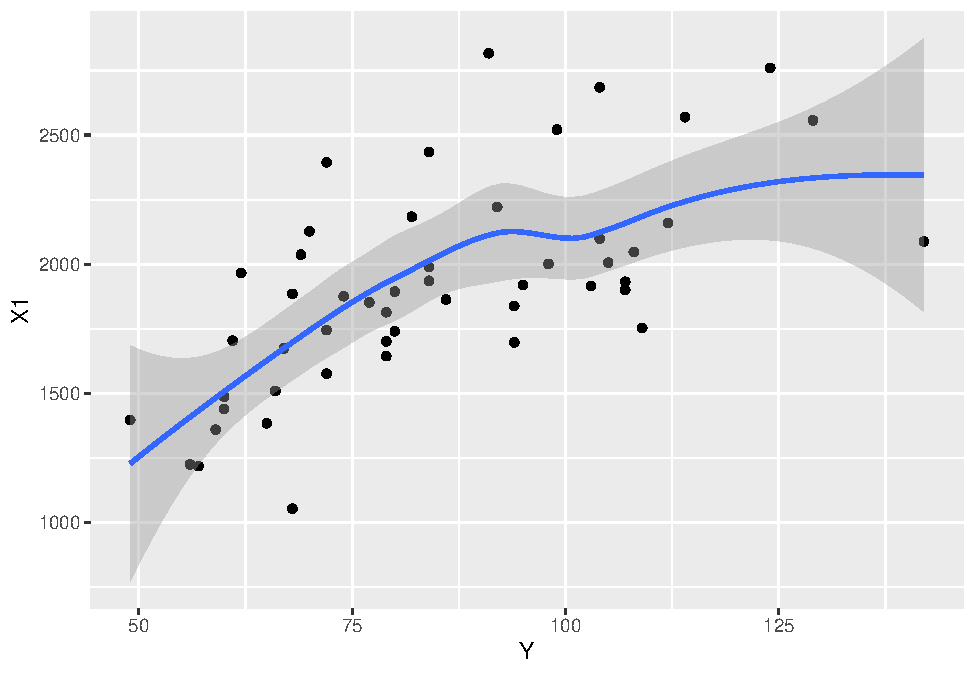
\includegraphics{PS_answers_files/figure-latex/unnamed-chunk-6-1.pdf}

\begin{Shaded}
\begin{Highlighting}[]
\CommentTok{#As per capita expenditure on public education increases, so does the relationship of per capita personal income. This is illustrated by the positive relationship drawn by the trendline. The relationship could be deemed correlational because having more people with more money, leads to more money going back into the system through taxes for example, to be spent on public education. Though one must note, ss per capita expenditure on public education passes approximately 100, the relationship becomes more neutral.}
\end{Highlighting}
\end{Shaded}

\#\#\#Number of residents per thousand under 18 years of age vs.~per
capita personal income

\begin{Shaded}
\begin{Highlighting}[]
\KeywordTok{ggplot}\NormalTok{(}\KeywordTok{aes}\NormalTok{(X1, X2), }\DataTypeTok{data=}\NormalTok{expenditure) }\OperatorTok{+}\StringTok{ }\CommentTok{#graphing each axis using variables within the expenditure data set}
\StringTok{  }\KeywordTok{geom_point}\NormalTok{() }\OperatorTok{+}\StringTok{ }\CommentTok{#adding points for each relationship}
\StringTok{  }\KeywordTok{geom_smooth}\NormalTok{() }\CommentTok{#adding a trendline}
\end{Highlighting}
\end{Shaded}

\begin{verbatim}
## `geom_smooth()` using method = 'loess' and formula 'y ~ x'
\end{verbatim}

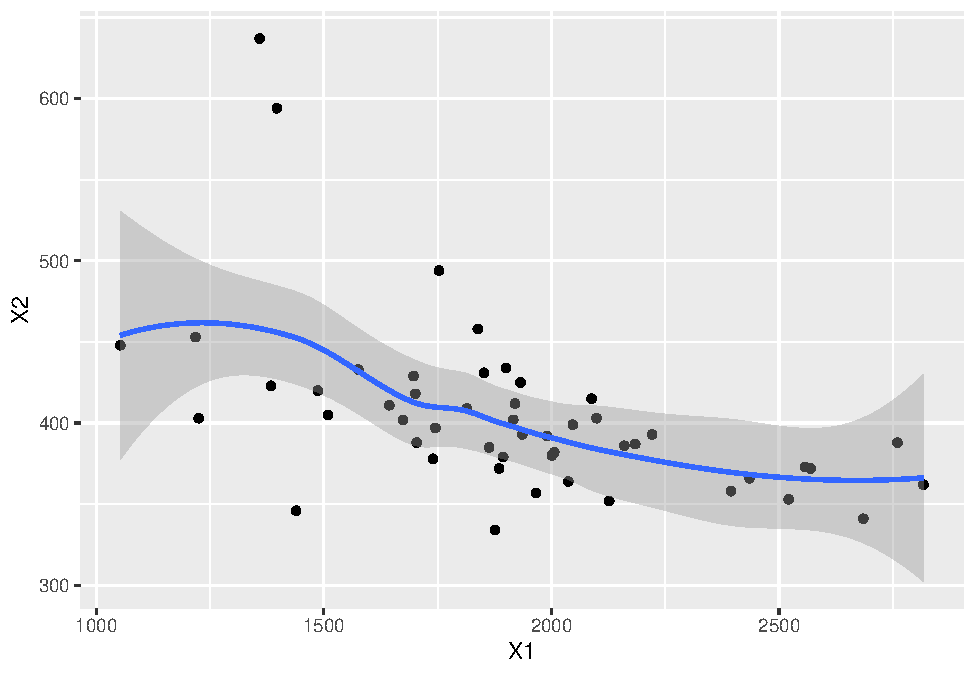
\includegraphics{PS_answers_files/figure-latex/unnamed-chunk-7-1.pdf}

\begin{Shaded}
\begin{Highlighting}[]
\CommentTok{#As per capita personal income increases, the number of residents per thousand under 18 years of age seem to decrease illustrated by the negative relationship indicated by the trendline. This makes sense, as one is more likely to earn more money later on in their life due to amass amounts of variables such as more educational experience, leading to higher paying jobs. }
\end{Highlighting}
\end{Shaded}

\hypertarget{number-of-people-per-thousand-residing-in-urban-areas-vs.-per-capita-personal-income}{%
\subsubsection{Number of people per thousand residing in urban areas
vs.~per capita personal
income}\label{number-of-people-per-thousand-residing-in-urban-areas-vs.-per-capita-personal-income}}

\begin{Shaded}
\begin{Highlighting}[]
\KeywordTok{ggplot}\NormalTok{(}\KeywordTok{aes}\NormalTok{(X1, X3), }\DataTypeTok{data=}\NormalTok{expenditure) }\OperatorTok{+}\StringTok{ }\CommentTok{#graphing each axis using variables within the expenditure data set}
\StringTok{  }\KeywordTok{geom_point}\NormalTok{() }\OperatorTok{+}\StringTok{ }\CommentTok{#adding points for each relationship}
\StringTok{  }\KeywordTok{geom_smooth}\NormalTok{() }\CommentTok{#adding a trendline}
\end{Highlighting}
\end{Shaded}

\begin{verbatim}
## `geom_smooth()` using method = 'loess' and formula 'y ~ x'
\end{verbatim}

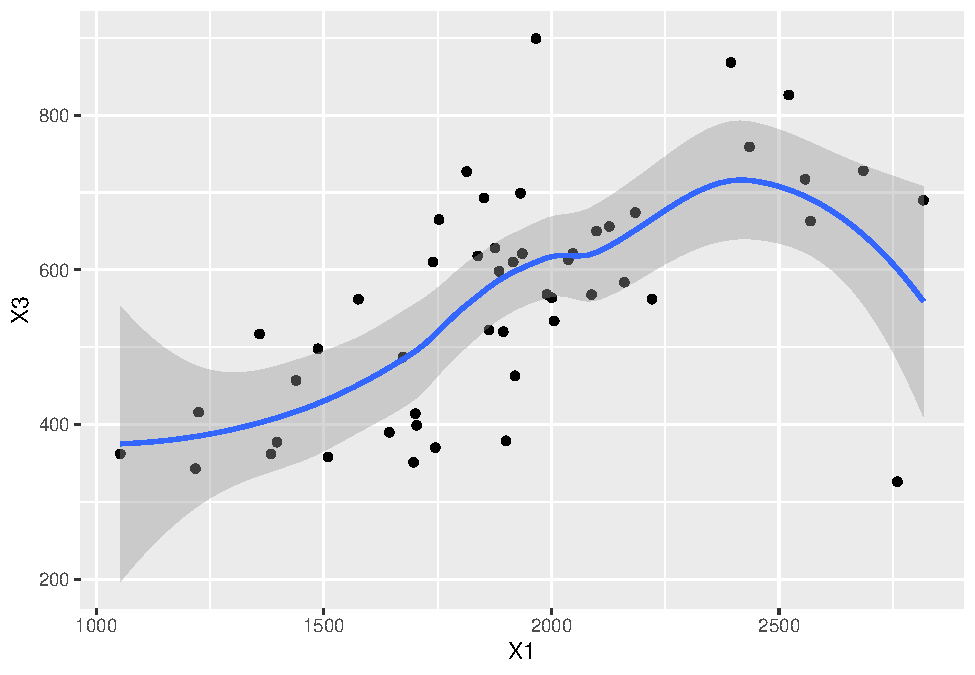
\includegraphics{PS_answers_files/figure-latex/unnamed-chunk-8-1.pdf}

\begin{Shaded}
\begin{Highlighting}[]
\CommentTok{#As per capita personal income increases, there is a general positive trend of the number of people per thousand residing in urban areas. This could be due to the fact that as personal income increases, one can afford to live in presumably better located residencies in urban areas, closer to work. That relationship because to decrease with the few observations around 2500 on 'X1' possibly because those who gain more money can afford even more luxurious locations outside of the urban areas. }
\end{Highlighting}
\end{Shaded}

\#\#Bullet 2

\hypertarget{per-capita-expenditure-on-public-education-vs.-region}{%
\subsubsection{Per capita expenditure on public education Vs.
Region}\label{per-capita-expenditure-on-public-education-vs.-region}}

\hypertarget{northeast-2-north-central-3-south-4-west}{%
\subparagraph{1 = Northeast \textbar{} 2 = North Central \textbar{} 3 =
South \textbar{} 4 =
West\textbar{}}\label{northeast-2-north-central-3-south-4-west}}

\begin{Shaded}
\begin{Highlighting}[]
\NormalTok{expenditure}\OperatorTok{$}\NormalTok{Region <-}\StringTok{ }\KeywordTok{as.factor}\NormalTok{(expenditure}\OperatorTok{$}\NormalTok{Region)}
\KeywordTok{ggplot}\NormalTok{(}\KeywordTok{aes}\NormalTok{(Region, Y), }\DataTypeTok{data=}\NormalTok{expenditure) }\OperatorTok{+}\StringTok{ }\CommentTok{#graphing each axis using variables within the expenditure data set}
\StringTok{  }\KeywordTok{geom_point}\NormalTok{(}\KeywordTok{aes}\NormalTok{(}\DataTypeTok{color =}\NormalTok{ Region)) }\CommentTok{#adding points for each relationship}
\end{Highlighting}
\end{Shaded}

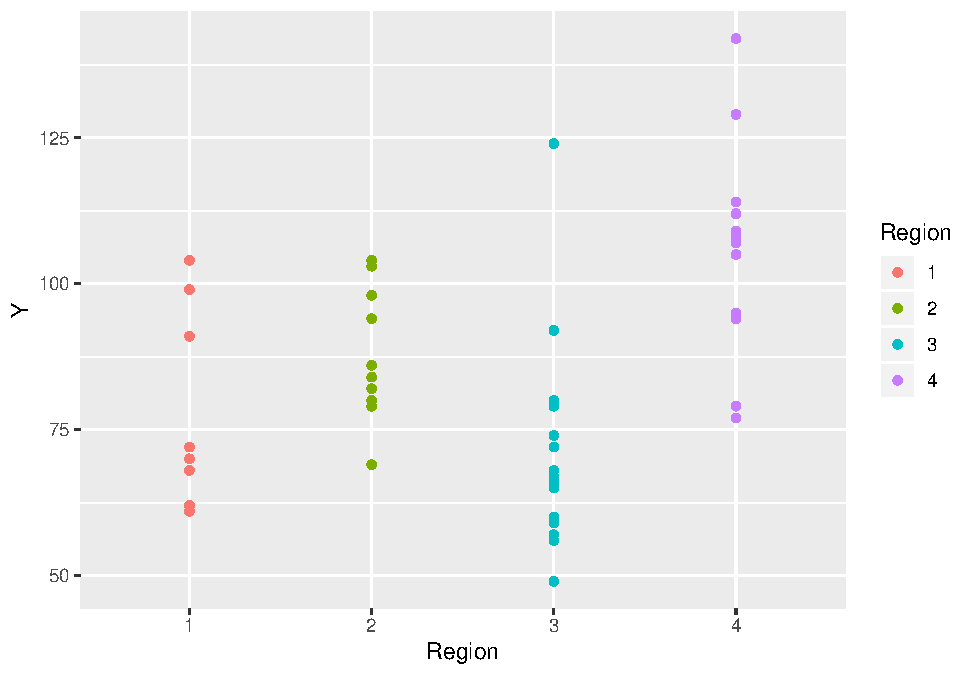
\includegraphics{PS_answers_files/figure-latex/unnamed-chunk-9-1.pdf}

\begin{Shaded}
\begin{Highlighting}[]
\CommentTok{#For each region, there are differences between the per capita expenditure on public education as indicated by the spread within the graph. On average, the South (Region 3), has the lowest expenditure; whereas the West (Region 4) has the highest expenditure on public education. The North Central region (Region 2) slightly edges out the Northeast (Region 1), but both exist in between the South and West's expenditures}
\end{Highlighting}
\end{Shaded}

\#\#Bullet 3 \#\#\#Per capita personal income vs.~Per capita expenditure
on public education relationship Based on Region

\begin{Shaded}
\begin{Highlighting}[]
\KeywordTok{ggplot}\NormalTok{(}\KeywordTok{aes}\NormalTok{(X1, Y), }\DataTypeTok{data=}\NormalTok{expenditure) }\OperatorTok{+}\StringTok{ }\CommentTok{#graphing each axis using variables within the expenditure data set}
\StringTok{  }\KeywordTok{geom_point}\NormalTok{(}\KeywordTok{aes}\NormalTok{(}\DataTypeTok{color =}\NormalTok{ Region, }\DataTypeTok{shape =}\NormalTok{ Region)) }\OperatorTok{+}\StringTok{ }\CommentTok{#adding points for each relationship}
\StringTok{  }\KeywordTok{facet_wrap}\NormalTok{(}\OperatorTok{~}\NormalTok{Region) }\CommentTok{#compartmentalizing per region}
\end{Highlighting}
\end{Shaded}

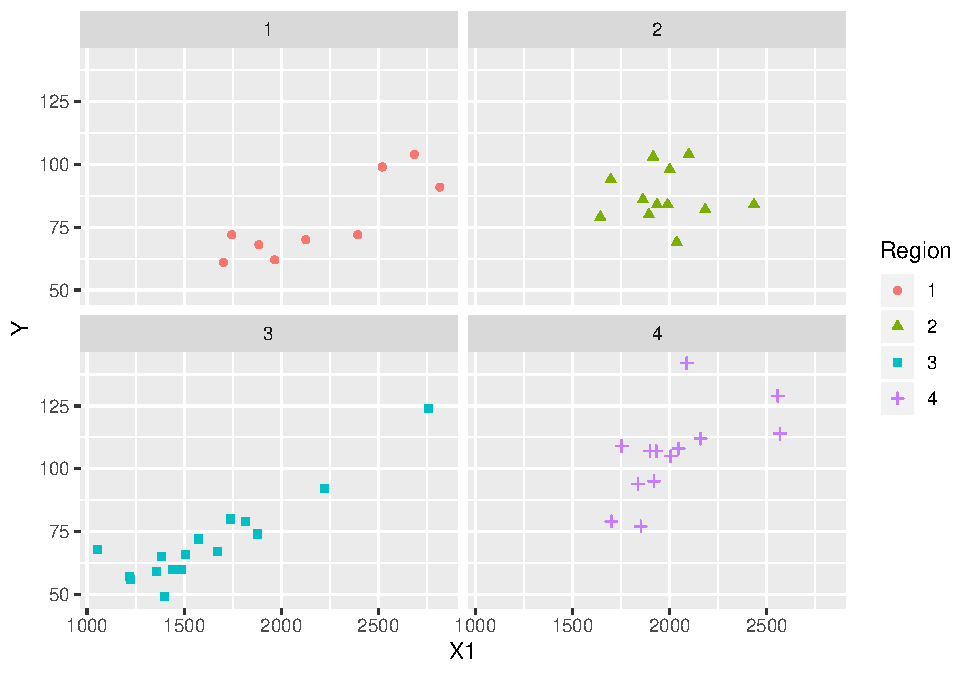
\includegraphics{PS_answers_files/figure-latex/unnamed-chunk-10-1.pdf}


\end{document}
